\begin{frame}
    \frametitle{Solutions}

    \begin{description}
        \item[Smooth solution] for both domains.
            \begin{gather}
                u(x, y) = \sin(2 \pi x) \cos(2 \pi y).
            \end{gather}
        \item[Low-regularity solution] for the square domain. 
            \begin{gather}
                u(x, y) = \frac{1 - e^{-100x}}{1 - e^{-100}} \sin(\pi y) (1 - x).
            \end{gather}
        \item[Low-regularity solution] for the L-shaped domain.
            \begin{gather}
                u(\rho, \theta) = \rho^{2 / 3} \sin\left(\frac{2 \theta}{3}\right).
            \end{gather}
    \end{description}
\end{frame}

\subsection{Uniform Refinement}

\begin{frame}[fragile]
    \frametitle{Errors}
    \framesubtitle{Square domain}

    \lstinline{./executables/square_smooth.out 3}

    \begin{figure}[!ht]
        % Errors v Size template for TikZ.

\begin{subfigure}[b]{0.45\textwidth}
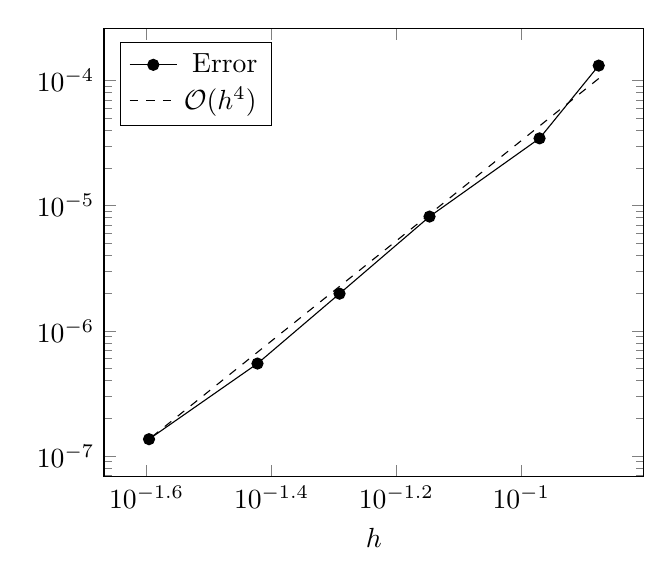
\begin{tikzpicture}
\begin{loglogaxis}[
    xlabel={$h$},
    legend pos=north west,
]

\addplot[black, mark=*] coordinates {(0.13307,0.000131393) (0.106989,3.44649e-05) (0.0713092,8.1769e-06) (0.0511671,1.98114e-06) (0.0378115,5.47747e-07) (0.0253431,1.36302e-07)};
\addlegendentry{$\LT$ Error}

\addplot[black, dashed] coordinates {(0.13307,0.0001036057614569891) (0.0253431,1.36302e-07)};
\addlegendentry{$\mathcal{O}(h^{4})$}

\end{loglogaxis}
\end{tikzpicture}
\end{subfigure}
\hfill
\begin{subfigure}[b]{0.45\textwidth}
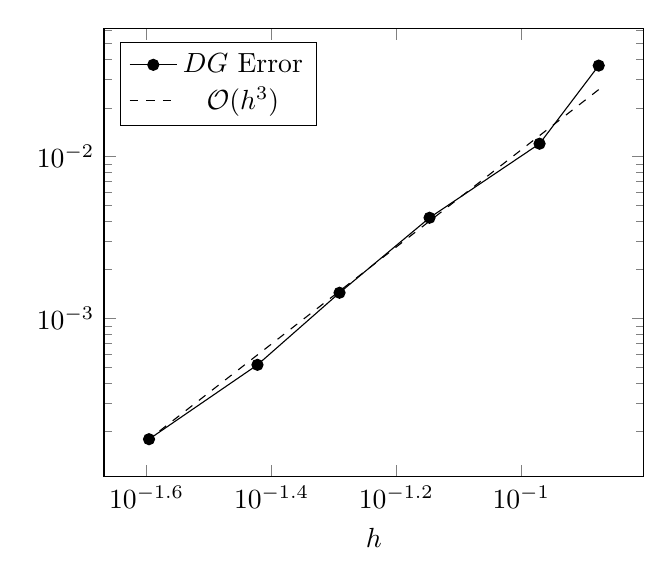
\begin{tikzpicture}
\begin{loglogaxis}[
    xlabel={$h$},
    legend pos=north west,
]

\addplot[black, mark=*] coordinates {(0.13307,0.036557) (0.106989,0.0120258) (0.0713092,0.00419264) (0.0511671,0.00144215) (0.0378115,0.000517054) (0.0253431,0.000179452)};
\addlegendentry{$DG$ Error}

\addplot[black, dashed] coordinates {(0.13307,0.025978230256595083) (0.0253431,0.000179452)};
\addlegendentry{$\mathcal{O}(h^{3})$}

\end{loglogaxis}
\end{tikzpicture}
\end{subfigure}
        \caption{$\LT$ and $DG$ errors versus mesh size on a sequence of uniform meshes over a square domain. $k = 3$, $N \in \{125, 250, \dots, 4000\}$.}
    \end{figure}
\end{frame}

\begin{frame}[fragile]
    \frametitle{Errors}
    \framesubtitle{L-shaped domain}

    \lstinline{./executables/lshape_smooth.out 3}

    \begin{figure}[!ht]
        % Errors v Size template for TikZ.

\begin{subfigure}[b]{0.45\textwidth}
\begin{tikzpicture}[scale=.6]
\begin{loglogaxis}[
    xlabel={$h$},
    legend pos=north west,
]

\addplot[solarized-base02, mark=*] coordinates {(0.236846,0.00236589) (0.162063,0.000476832) (0.125487,0.000110835) (0.0834066,2.72149e-05) (0.0598985,6.75002e-06) (0.0458041,1.74035e-06)};
\addlegendentry{$\LT$ Error}

\addplot[solarized-base02, dashed] coordinates {(0.236846,0.0012441805245544592) (0.0458041,1.74035e-06)};
\addlegendentry{$\mathcal{O}(h^{4})$}

\end{loglogaxis}
\end{tikzpicture}
\end{subfigure}
\hfill
\begin{subfigure}[b]{0.45\textwidth}
\begin{tikzpicture}[scale=.6]
\begin{loglogaxis}[
    xlabel={$h$},
    legend pos=north west,
]

\addplot[solarized-base02, mark=*] coordinates {(0.236846,0.354304) (0.162063,0.112679) (0.125487,0.0379581) (0.0834066,0.0128848) (0.0598985,0.00442298) (0.0458041,0.0015715)};
\addlegendentry{$DG$ Error}

\addplot[solarized-base02, dashed] coordinates {(0.236846,0.2172698609297559) (0.0458041,0.0015715)};
\addlegendentry{$\mathcal{O}(h^{3})$}

\end{loglogaxis}
\end{tikzpicture}
\end{subfigure}
        \caption{$\LT$ and $DG$ errors versus mesh size on a sequence of uniform meshes over an L-shaped domain. $k = 3$, $N \in \{125, 250, \dots, 4000\}$.}
    \end{figure}
\end{frame}

\begin{frame}
    \frametitle{Meshes}

    \begin{figure}[!ht]
        \centering
        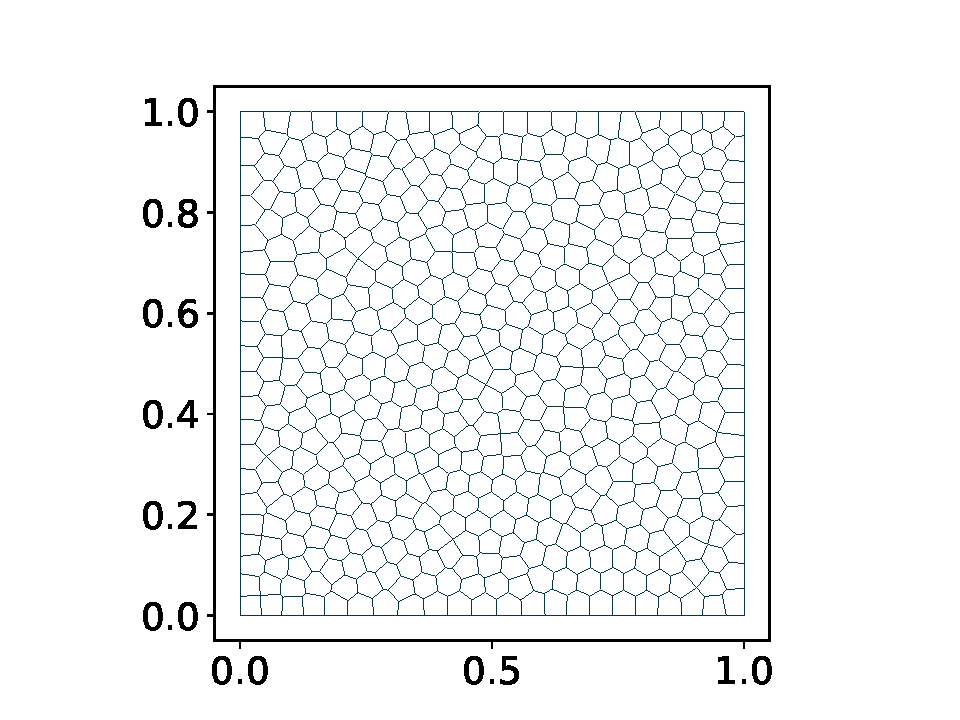
\includegraphics[trim=1cm 0.5cm 1cm 0.5cm, clip, width=0.275\textwidth]{meshes/uniform/square_500.pdf}
        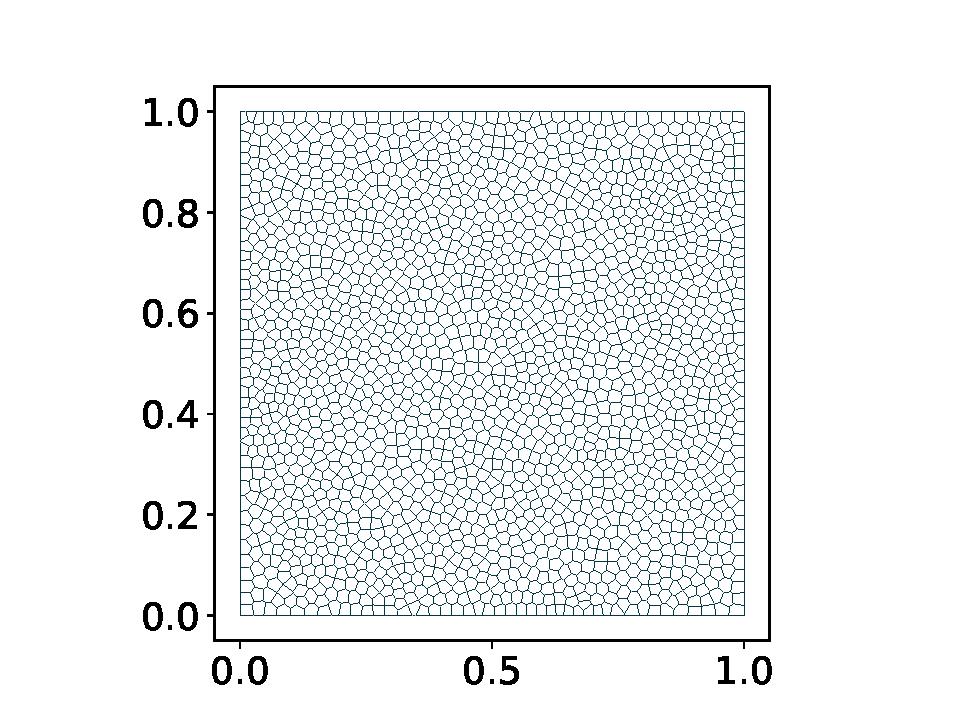
\includegraphics[trim=1cm 0.5cm 1cm 0.5cm, clip, width=0.275\textwidth]{meshes/uniform/square_2000.pdf}
        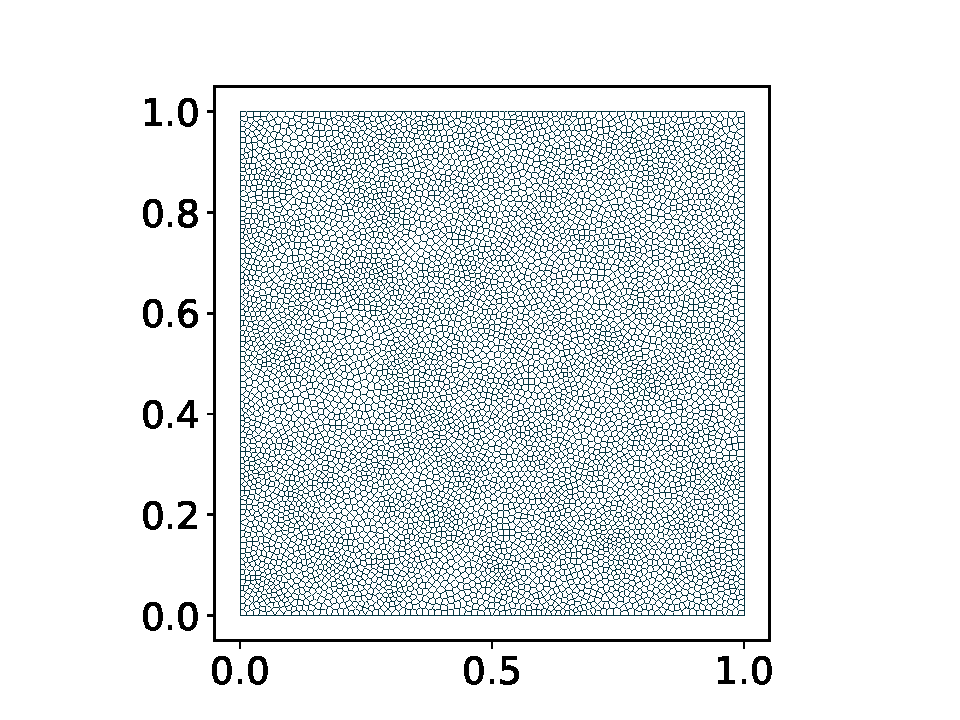
\includegraphics[trim=1cm 0.5cm 1cm 0.5cm, clip, width=0.275\textwidth]{meshes/uniform/square_8000.pdf}
        \caption{Square uniform meshes, with $N \in \{500, 2000, 8000\}$.}
    \end{figure}

    \begin{figure}[!ht]
        \centering
        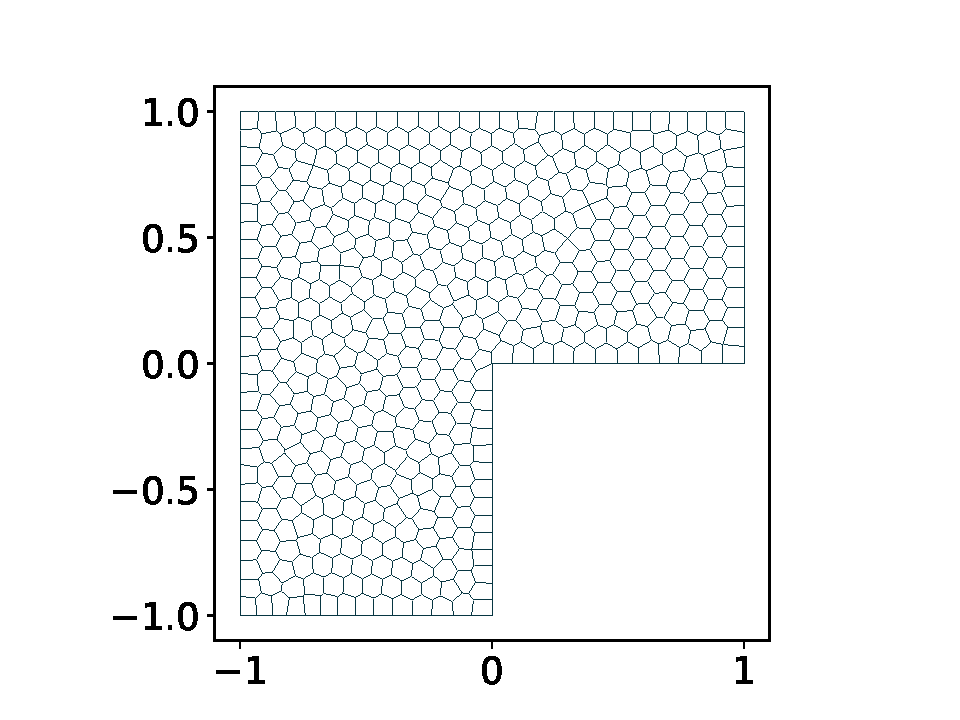
\includegraphics[trim=1cm 0.5cm 1cm 0.5cm, clip, width=0.275\textwidth]{meshes/uniform/lshape_500.pdf}
        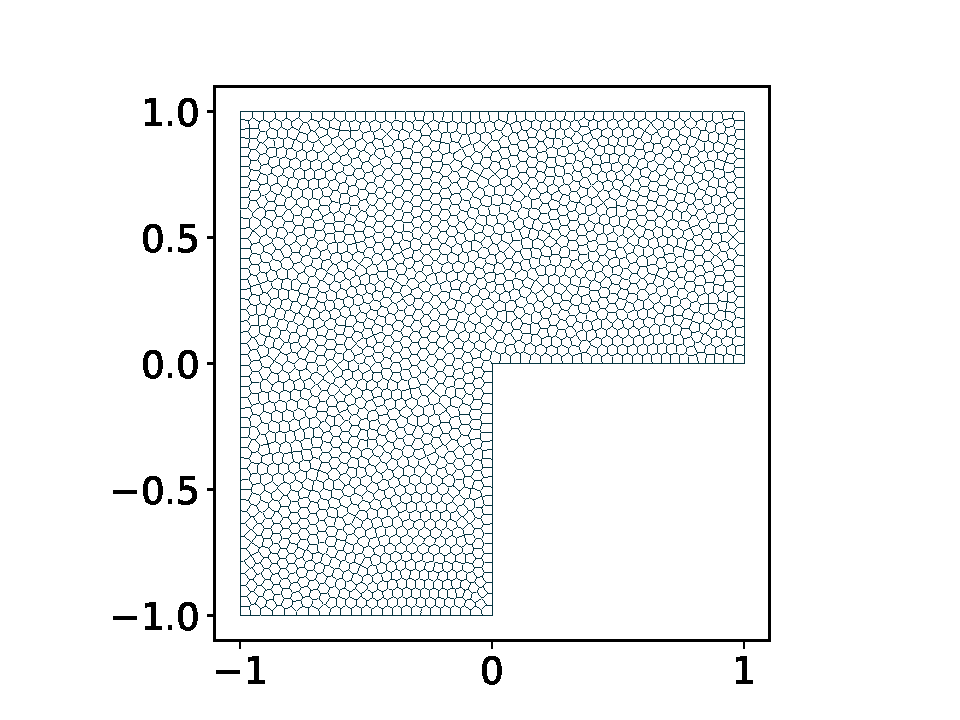
\includegraphics[trim=1cm 0.5cm 1cm 0.5cm, clip, width=0.275\textwidth]{meshes/uniform/lshape_2000.pdf}
        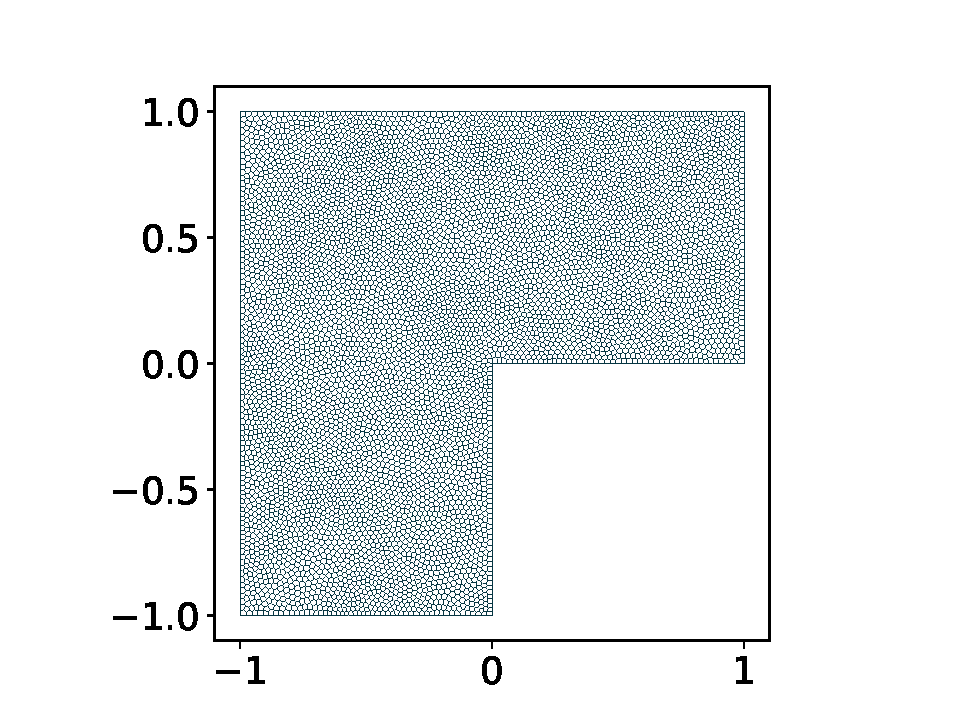
\includegraphics[trim=1cm 0.5cm 1cm 0.5cm, clip, width=0.275\textwidth]{meshes/uniform/lshape_8000.pdf}
        \caption{L-shaped uniform meshes, with $N \in \{500, 2000, 8000\}$.}
    \end{figure}
\end{frame}

\subsection{Uniform Refinement Versus \textit{h-Adaptive} Refinement}

\subsection{\textit{h-adaptive} Refinement Versus \textit{hp-Adaptive} Refinement}